\documentclass[11pt,a4paper]{article}

% -----------------------------------------------------------------------------
% CS6868 Research Mini-Project Report Template
% -----------------------------------------------------------------------------
% Target length: 5-10 pages (including figures, excluding references).
% Compile with: latexmk -pdf main.tex
% -----------------------------------------------------------------------------

\usepackage[utf8]{inputenc}
\usepackage[T1]{fontenc}
\usepackage[margin=1in]{geometry}
\usepackage{microtype}
\usepackage{lmodern}
\usepackage{amsmath,amssymb}
\usepackage{graphicx}
\usepackage{subcaption}
\usepackage{booktabs}
\usepackage{array}
\usepackage{enumitem}
\usepackage{xcolor}
\usepackage{listings}
\usepackage{hyperref}
\usepackage[capitalise,noabbrev]{cleveref}
\usepackage{minted}
\usepackage[section]{placeins}
\usepackage{tabularx}
\usepackage{pgfplots}
\pgfplotsset{compat=1.18}

% --- Drafting markers (remove before submission) -----------------------------
% \rebench{x}: a number that must be re-measured with the final benchmarking method
\newcommand{\rebench}[1]{\textcolor{red}{#1}}

\hypersetup{
  colorlinks=true,
  linkcolor=black,
  citecolor=blue!60!black,
  urlcolor=blue!60!black,
}

% --- Listings style (for code snippets) ---------------------------------------
\definecolor{codegray}{gray}{0.95}
\lstset{
  basicstyle=\ttfamily\small,
  backgroundcolor=\color{codegray},
  frame=single,
  framesep=4pt,
  breaklines=true,
  columns=fullflexible,
  keepspaces=true,
  showstringspaces=false,
}

% --- Title block --------------------------------------------------------------
\title{%
  \textbf{CS6023 Course Project} \\[0.3em]
  \Large CUDA Ray Tracing
}
\author{%
  Ventrapragada Krishna Sameer \\ \texttt{cs23b078@smail.iitm.ac.in}
}
\date{\today}

\begin{document}
\maketitle

\begin{abstract}

The main goal of this project is to build a working ray tracer in CUDA, add reflections and shadows, then make it faster. We start with a basic CPU ray tracer that renders 3 spheres on a checkerboard
floor with diffuse shading and hard shadows. We first port it to CUDA and then extend it to multiple reflections with multiple spheres. The report provides all the optimizations we did.

\end{abstract}

% =============================================================================
\section{Introduction}
\label{sec:intro}

Ray tracing computes the colour of every pixel by following a ray from the camera into the scene,
finding the closest object it hits, and shading that point; shadows and reflections need further
rays. Every pixel is independent, which makes the problem naturally parallel, but the work per pixel
varies: a ray that sees the sky stops at once, a ray that keeps hitting mirrors bounces many times.
This irregular control flow makes it an interesting GPU workload.

The project follows the brief in three stages: port the CPU ray tracer to CUDA (\cref{sec:port}),
add multiple reflection bounces and study how the time scales with depth and resolution
(\cref{sec:multibounce}), and scale the scene to 5,000 spheres and make the kernel faster
(\cref{sec:scene,sec:opt,sec:failed}). Each optimization follows the same loop: profile, form a
hypothesis, change one thing, measure again. \Cref{sec:discussion} discusses divergence, occupancy,
register pressure and memory behaviour; \cref{sec:bvh} briefly covers a bounding volume hierarchy as
an algorithmic extension.

% =============================================================================
\section{Setup and measurement method}
\label{sec:method}

All measurements use an NVIDIA Tesla T4 (Turing, 40 SMs) on Google Colab, \texttt{nvcc} 13.0 with
\texttt{-O2}, Nsight Systems and Nsight Compute 2025.3.1, an $800 \times 600$ image, reflection
depth 10 and energy threshold 0.01 unless stated otherwise.

\paragraph{Timing.} Only the kernel is timed, with CUDA events. Every program first runs one untimed
launch of the same kernel and synchronizes, then times a second launch. Without this in-process
warm-up, the first launch in each process waited $\approx$173\,$\mu$s for the kernel code to be
loaded (seen in Nsight Systems), which dominated sub-millisecond measurements. Every data point is the
mean of 10 runs. Times vary between Colab sessions by up to 7\,\%, so versions are only compared
within one session, and the overview table runs all versions interleaved.

\paragraph{Correctness.} Every version's image is compared pixel by pixel with the baseline's; all
are identical except the two that change the arithmetic (\cref{sec:fma,sec:fp16}).

\paragraph{Profiles.} Nsight Compute (ncu) locks the SM clock at 585\,MHz (boost: up to 1590\,MHz),
so it measures the work a kernel needs, independent of the clock. Its durations are only compared
with each other; \cref{sec:blocks} shows a case where profile and timing disagree.

% =============================================================================
\section{Porting the CPU ray tracer to CUDA}
\label{sec:port}

The starter program renders 3 spheres on a checkerboard floor (itself a sphere of radius 1000): for
every pixel it finds the closest sphere hit by the camera ray, computes diffuse plus ambient light,
and casts one shadow ray. The port uses \textbf{one thread per pixel} on a 2D grid:
\begin{lstlisting}[language=C++]
int px = blockIdx.x * blockDim.x + threadIdx.x;
int py = blockIdx.y * blockDim.y + threadIdx.y;
if (px >= W || py >= H) return;      // the grid is rounded up to whole blocks
\end{lstlisting}
The first version uses $32 \times 32$ blocks, a grid of $25 \times 19$ blocks; the last block row has
8 rows of idle threads, handled by the bounds check. A warp is 32 consecutive \texttt{threadIdx.x},
so with 32-wide blocks \textbf{one warp is one row of 32 pixels}, which matters for divergence later.
The scene is copied to the GPU once, the image back once. The GPU image matches the CPU's except for
4 pixels that differ by 1/255 (the GPU fuses \texttt{a*b+c} into one FMA instruction).

\begin{table}[h]
  \centering
  \begin{tabular}{@{}lr@{}}
    \toprule
    $800 \times 600$, 3 spheres & Time \\
    \midrule
    CPU, \texttt{g++ -O2}, one thread (whole process) & 53.5\,ms \\
    GPU kernel (CUDA events) & \textbf{0.042\,ms} \\
    GPU, whole process & 248.9\,ms \\
    \bottomrule
  \end{tabular}
  \caption{CPU vs.\ GPU on the starter scene. The CPU program has no internal timer, so its time
    includes process start and writing the image.}
  \label{tab:cpugpu}
\end{table}

The kernel is $\approx$\textbf{1,300$\times$} faster than the CPU loop, but the GPU program as a whole
is five times slower: almost all of its 249\,ms is CUDA context creation (the first
\texttt{cudaMalloc} alone takes $\approx$180\,ms). A three-sphere scene is too small to study GPU
efficiency, so the rest of the project uses larger scenes and times only the kernel.

% =============================================================================
\section{Multiple reflection bounces}
\label{sec:multibounce}

The colour along a ray is the local shading plus $k$ times the colour along the reflected ray
($k$: reflectivity). Recursion is a poor fit for a GPU (small per-thread stack, different depth per
thread), so the bounce chain is a loop that carries the ray's remaining \textbf{energy}:
\begin{lstlisting}[language=C++]
float curr = 1;                          // how much this bounce still contributes
do {
    depth--;
    hit = closestHit(origin, dir, ...);
    if (hit < 0) { color += sky(dir) * curr; break; }   // the ray leaves the scene
    ... local shading and shadow ray ...
    color = color + local * curr * (1.0f - k);
    curr *= k;
    origin = p + n * 0.001f;             // start slightly off the surface
    dir = normalize(dir - n * 2 * dot(dir, n));          // r = d - 2 (d.n) n
} while (depth >= 0 && curr > threshold);
\end{lstlisting}
A ray stops at the maximum depth, when it sees the sky, or when its energy drops below the threshold.
Shadow rays only need to know \emph{whether} something blocks the light, so their search returns at
the first hit.

\subsection{Scaling with the bounce depth}
\label{sec:depth}

\begin{figure}[h]
  \centering
  \begin{tikzpicture}
    \begin{axis}[width=0.75\linewidth, height=5cm, xlabel={maximum reflection depth},
                 ylabel={kernel time (ms)}, grid=major, legend pos=north west,
                 legend style={font=\scriptsize}, xtick={0,...,10}]
      \addplot+[mark=*] table[col sep=comma, x=depth, y=timed_32x32]
        {results/final/scene/compare_depth_N400_t0.csv};
      \addlegendentry{baseline, no threshold}
      \addplot+[mark=*, dashed] table[col sep=comma, x=depth, y=timed_32x32]
        {results/final/scene/compare_depth_N400_t0.01.csv};
      \addlegendentry{baseline, threshold 0.01}
      \addplot+[mark=square*] table[col sep=comma, x=depth, y=fma_8x8]
        {results/final/scene/compare_depth_N400_t0.csv};
      \addlegendentry{best, no threshold}
      \addplot+[mark=square*, dashed] table[col sep=comma, x=depth, y=fma_8x8]
        {results/final/scene/compare_depth_N400_t0.01.csv};
      \addlegendentry{best, threshold 0.01}
    \end{axis}
  \end{tikzpicture}
  \caption{Kernel time against the maximum reflection depth, 400 spheres. ``Baseline'': first
    multi-bounce version; ``best'': final version of \cref{sec:opt}.}
  \label{fig:depthplot}
\end{figure}

With the threshold, the time stops growing at depth 5: by then the threshold or a sky miss has
stopped almost every ray (\cref{fig:depthplot}). Without it, the time keeps growing, but each level
costs less (+0.58\,ms for depth 1, +0.09\,ms for depth 10), since rays still stop at the sky or at
fully diffuse surfaces; at depth 10 the threshold saves 25--30\,\%. The speedup of the optimized
version grows with depth (1.29--1.38$\times$ at depth 0, 1.47--1.58$\times$ at depth 10): deeper bounces
make the work per pixel more uneven, which the block change of \cref{sec:blocks} reduces. Visually
(\cref{fig:depth}), depth 1 changes 45\,\% of the pixels, depths 2 and 3 another 19\,\% and 7\,\%;
from depth 4 the changes are invisible.

\begin{figure}[h]
  \centering
  \begin{subfigure}{0.24\linewidth}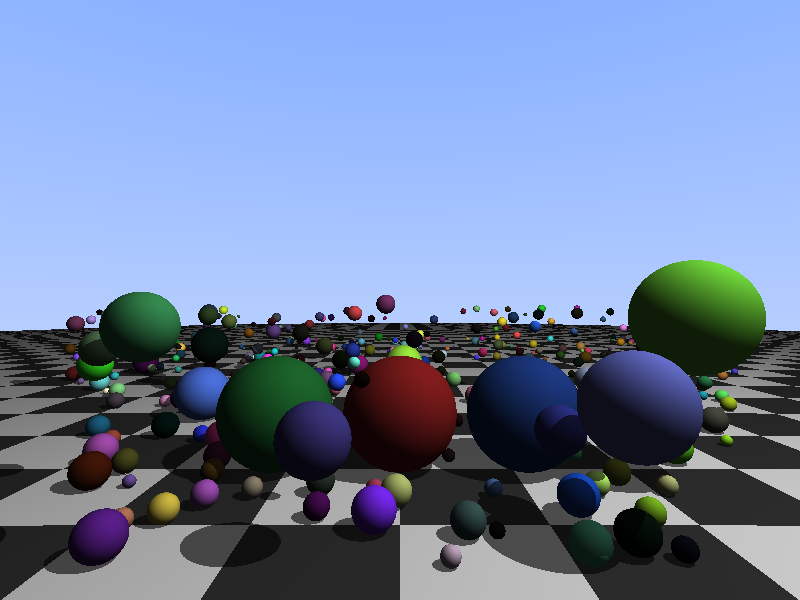
\includegraphics[width=\linewidth]{results/depth_images/depth_0.png}\caption{depth 0}\end{subfigure}\hfill
  \begin{subfigure}{0.24\linewidth}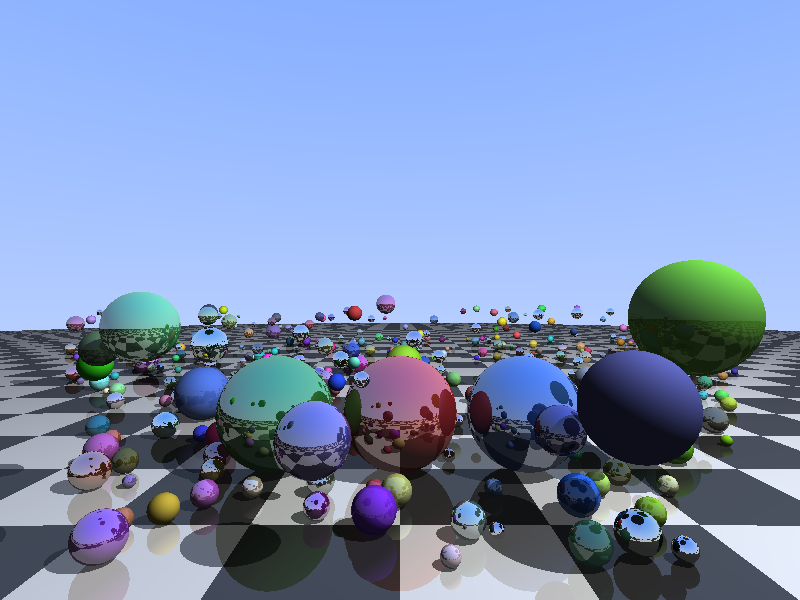
\includegraphics[width=\linewidth]{results/depth_images/depth_1.png}\caption{depth 1}\end{subfigure}\hfill
  \begin{subfigure}{0.24\linewidth}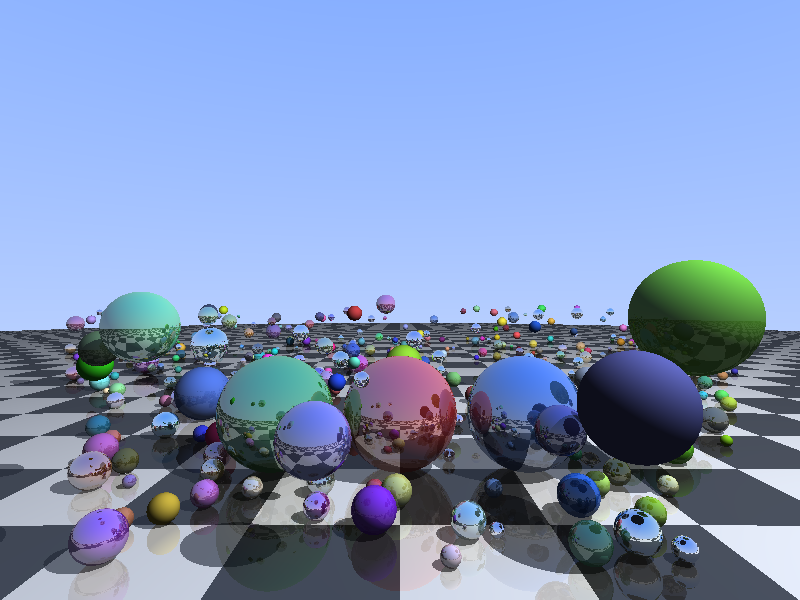
\includegraphics[width=\linewidth]{results/depth_images/depth_3.png}\caption{depth 3}\end{subfigure}\hfill
  \begin{subfigure}{0.24\linewidth}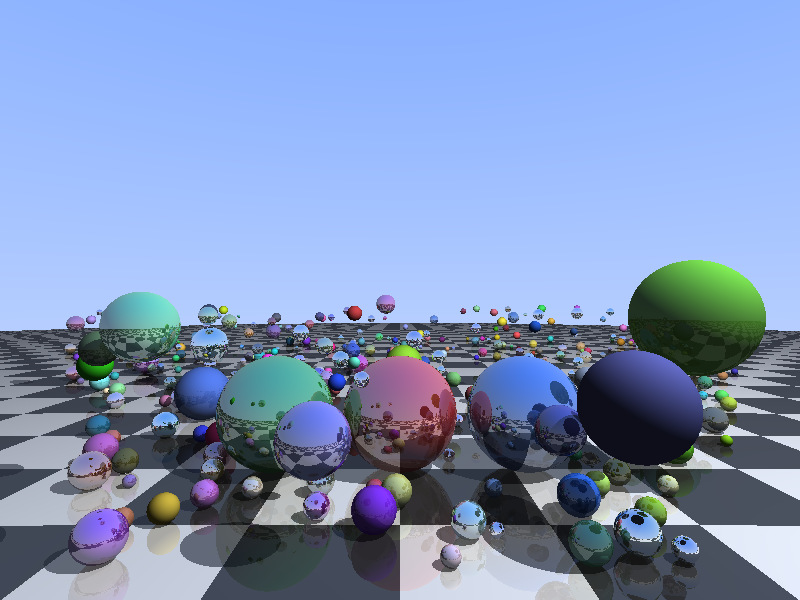
\includegraphics[width=\linewidth]{results/depth_images/depth_10.png}\caption{depth 10}\end{subfigure}
  \caption{The same scene (400 spheres) at increasing maximum reflection depth.}
  \label{fig:depth}
\end{figure}

\subsection{Scaling with the image resolution}
\label{sec:resolution}

\begin{figure}[h]
  \centering
  \begin{tikzpicture}
    \begin{semilogxaxis}[width=0.75\linewidth, height=5cm, xlabel={megapixels},
                 ylabel={ms per megapixel}, grid=major, legend pos=north east,
                 legend style={font=\scriptsize}, ymin=0]
      \addplot+[mark=*] table[col sep=comma, x=Mpix, y=timed_32x32_ms_per_mpix]
        {results/final/scene/compare_resolution_N400.csv};
      \addlegendentry{baseline}
      \addplot+[mark=square*] table[col sep=comma, x=Mpix, y=fma_8x8_ms_per_mpix]
        {results/final/scene/compare_resolution_N400.csv};
      \addlegendentry{best}
    \end{semilogxaxis}
  \end{tikzpicture}
  \caption{Cost per megapixel from $320 \times 240$ to $3200 \times 2400$ (all 4:3, same view),
    400 spheres.}
  \label{fig:resplot}
\end{figure}

Small images are inefficient (\cref{fig:resplot}): $320 \times 240$ has only $\approx$2,400 warps
while a T4 holds 1,280 at once, so fewer than two ``waves'' of work leave SMs idle at the end
(13.6 vs.\ 7.2\,ms per megapixel at 1--2 megapixels). Between 1 and 2 megapixels the time is linear
in the pixel count. The largest images cost more per pixel again (9.0\,ms at $3200 \times 2400$);
their 50--70\,ms kernels likely run at a lower clock (\cref{sec:blocks}). The speedup of the
optimizations holds at every size (1.35--1.59$\times$).

% =============================================================================
\section{Scaling the scene}
\label{sec:scene}

With 3 spheres the kernel is too short to study, so the scene was extended to \textbf{5,000
spheres} (20 hand-placed, the rest small and random); every program renders the floor plus the first
$N$ spheres. Since every ray tests every sphere, the time grows linearly with $N$, at
$\approx$0.01\,ms per sphere up to $\approx$1,400 spheres (\cref{fig:sizes}). The profile at 400
spheres shows the scene in L1 (hit rate 99.9\,\%) and, in the machine code, \textbf{four separate
32-bit loads} per sphere test: the 36-byte \texttt{Sphere} struct is only 4-byte aligned, so the
compiler cannot use one wide load.

Above $\approx$1,400 spheres the cost per sphere rises steeply and settles at $\approx$0.019\,ms
for large $N$ (\cref{fig:sizes}, right). Each SM has 64\,KB of L1 cache here, and 1,819 spheres
$\times$ 36 bytes $\approx$ 64\,KB: beyond that, every scan of the sphere list misses L1 and is
served from L2. At 5,000 spheres L2 traffic is $\approx$150$\times$ that at 400, and all of the extra
time is memory stalls (waiting for missed loads, a full load queue), while L2 bandwidth stays almost
unused (0.3\,\%): the kernel waits for data, it is not short of bandwidth.

\begin{figure}[h]
  \centering
  \begin{tikzpicture}
    \begin{axis}[width=0.49\linewidth, height=5cm, xlabel={spheres $N$}, ylabel={kernel time (ms)},
                 grid=major, legend pos=north west, legend style={font=\scriptsize},
                 unbounded coords=jump, scaled x ticks=false]
      \addplot+[mark=*, mark size=1.5pt] table[col sep=comma, x=N, y=base]
        {results/final/scene/sizes_split_vs_timed.csv};
      \addlegendentry{baseline}
      \addplot+[mark=square*, mark size=1.5pt] table[col sep=comma, x=N, y=opt]
        {results/final/scene/sizes_split_vs_timed.csv};
      \addlegendentry{split (\cref{sec:split})}
      \addplot+[mark=triangle*, mark size=1.5pt] table[col sep=comma, x=N, y=opt]
        {results/final/scene/sizes_shared_vs_timed.csv};
      \addlegendentry{shared (\cref{sec:shared})}
    \end{axis}
  \end{tikzpicture}\hfill
  \begin{tikzpicture}
    \begin{axis}[width=0.49\linewidth, height=5cm, xlabel={spheres $N$},
                 ylabel={$\mu$s per extra sphere}, grid=major, legend pos=north west,
                 legend style={font=\scriptsize}, unbounded coords=jump, scaled x ticks=false]
      \addplot+[mark=*, mark size=1.5pt] table[col sep=comma, x=N, y expr=1000*\thisrow{base_ms_per_sphere}]
        {results/final/scene/sizes_split_vs_timed.csv};
      \addlegendentry{baseline}
      \addplot+[mark=square*, mark size=1.5pt] table[col sep=comma, x=N, y expr=1000*\thisrow{opt_ms_per_sphere}]
        {results/final/scene/sizes_split_vs_timed.csv};
      \addlegendentry{split}
      \addplot+[mark=triangle*, mark size=1.5pt] table[col sep=comma, x=N, y expr=1000*\thisrow{opt_ms_per_sphere}]
        {results/final/scene/sizes_shared_vs_timed.csv};
      \addlegendentry{shared}
    \end{axis}
  \end{tikzpicture}
  \caption{Kernel time (left) and cost of each additional sphere (right) against $N$, $32 \times 32$
    blocks. The baseline's 36-byte spheres stop fitting in L1 at $\approx$1,800, the split
    version's 16-byte spheres at $\approx$3,800--4,000; shared memory holds at most 1,819.}
  \label{fig:sizes}
\end{figure}

% =============================================================================
\section{GPU-side optimizations}
\label{sec:opt}

\Cref{tab:all} gives every step at 5,000 spheres, measured interleaved in one session on the main
scene and on two other 5,000-sphere scenes (tiny sparse spheres; larger, less reflective spheres).

\begin{table}[h]
  \centering
  \begin{tabular}{@{}llrrrr@{}}
    \toprule
    & & \multicolumn{3}{c}{kernel time (ms)} & ncu (ms) \\
    \cmidrule(lr){3-5}\cmidrule(l){6-6}
    version & block & main & sparse & large & main \\
    \midrule
    baseline                                   & $32 \times 32$ & 84.1 & 86.4 & 73.3 & 184.8 \\
    split (\cref{sec:split})                   & $32 \times 32$ & 67.5 & 67.8 & 60.2 & 155.5 \\
    split (\cref{sec:blocks})                  & $8 \times 8$   & 54.8 & 46.1 & 52.5 & 112.0 \\
    + fewer FP instructions (\cref{sec:fma})   & $8 \times 8$   & \textbf{51.2} & \textbf{42.4} & \textbf{48.7} & 106.0 \\
    \midrule
    \multicolumn{2}{@{}l}{total speedup} & \textbf{1.64$\times$} & \textbf{2.04$\times$} & \textbf{1.50$\times$} & 1.74$\times$ \\
    \midrule
    two spheres per iteration (\cref{sec:failed}) & $8 \times 8$ & 56.3 & 47.8 & 54.3 & 114.6 \\
    software prefetch (\cref{sec:failed})         & $8 \times 8$ & 58.9 & 49.9 & 57.6 & 114.1 \\
    \bottomrule
  \end{tabular}
  \caption{All flat versions at 5,000 spheres, depth 10, threshold 0.01: mean of 10 interleaved runs
    (std.\ 0.5--1.6\,ms), and the ncu duration at 585\,MHz. The last two rows are variants of the
    $8 \times 8$ split version that did not help.}
  \label{tab:all}
\end{table}

\Cref{fig:sweep} repeats the same interleaved measurement for scene sizes from 400 to 5,000 spheres.
\rebench{[Describe the trend once the sweep is in.]}

\IfFileExists{results/final/scene/sweep_all.csv}{
\begin{figure}[h]
  \centering
  \pgfplotsset{sweep/.style={width=0.49\linewidth, height=5.5cm, xlabel={spheres $N$}, grid=major,
               legend style={font=\scriptsize}, scaled x ticks=false, unbounded coords=jump,
               every axis plot/.append style={mark size=1.5pt}}}
  \begin{tikzpicture}
    \begin{axis}[sweep, ylabel={kernel time (ms)}, legend pos=north west]
      \addplot+[mark=*]        table[col sep=comma, x=N, y=timed_32x32]    {results/final/scene/sweep_all.csv};
      \addlegendentry{baseline $32 \times 32$}
      \addplot+[mark=square*]  table[col sep=comma, x=N, y=split_32x32]    {results/final/scene/sweep_all.csv};
      \addlegendentry{split $32 \times 32$}
      \addplot+[mark=triangle*] table[col sep=comma, x=N, y=split_8x8]     {results/final/scene/sweep_all.csv};
      \addlegendentry{split $8 \times 8$}
      \addplot+[mark=x, dashed] table[col sep=comma, x=N, y=2sphere_8x8]   {results/final/scene/sweep_all.csv};
      \addlegendentry{two spheres}
      \addplot+[mark=+, dashed] table[col sep=comma, x=N, y=prefetch_8x8]  {results/final/scene/sweep_all.csv};
      \addlegendentry{prefetch}
      \addplot+[mark=diamond*] table[col sep=comma, x=N, y=fma_8x8]        {results/final/scene/sweep_all.csv};
      \addlegendentry{fewer FP instr.}
    \end{axis}
  \end{tikzpicture}\hfill
  \begin{tikzpicture}
    \begin{axis}[sweep, ylabel={speedup over baseline}, legend pos=south east, cycle list shift=1]
      \addplot+[mark=square*]   table[col sep=comma, x=N, y=split_32x32_speedup]   {results/final/scene/sweep_all.csv};
      \addlegendentry{split $32 \times 32$}
      \addplot+[mark=triangle*] table[col sep=comma, x=N, y=split_8x8_speedup]     {results/final/scene/sweep_all.csv};
      \addlegendentry{split $8 \times 8$}
      \addplot+[mark=x, dashed] table[col sep=comma, x=N, y=2sphere_8x8_speedup]   {results/final/scene/sweep_all.csv};
      \addlegendentry{two spheres}
      \addplot+[mark=+, dashed] table[col sep=comma, x=N, y=prefetch_8x8_speedup]  {results/final/scene/sweep_all.csv};
      \addlegendentry{prefetch}
      \addplot+[mark=diamond*]  table[col sep=comma, x=N, y=fma_8x8_speedup]       {results/final/scene/sweep_all.csv};
      \addlegendentry{fewer FP instr.}
    \end{axis}
  \end{tikzpicture}
  \caption{All flat versions against the scene size (main scene, depth 10, threshold 0.01, mean of 10
    interleaved runs per point): kernel time (left) and speedup over the $32 \times 32$ baseline
    (right). Dashed: the two attempts of \cref{sec:failed}.}
  \label{fig:sweep}
\end{figure}
}{\rebench{[Figure fig:sweep: run sweep\_all.sh and copy results/sweep\_all.csv to results/final/scene/.]}}

\subsection{Scene in shared memory}
\label{sec:shared}

Each block copies the scene into shared memory once, synchronizes, and then reads only the shared
copy. A block may use 64\,KB of shared memory, i.e.\ at most \textbf{1,819 spheres}. The compiler now
emits one 128-bit shared load per sphere instead of four 32-bit global loads (6.6\,\% fewer
instructions), but while the scene fits in L1 the gain is small (1.06--1.11$\times$): on Turing, L1
and shared memory are the same SRAM. Near the baseline's L1 cliff it reaches 1.53$\times$ at 1,819
spheres, since shared memory is never evicted (\cref{fig:sizes}). Because of the size limit it is not
used further.

\subsection{Separating the data the intersection test needs}
\label{sec:split}

The intersection test only needs the centre and the radius, 16 of the 36 bytes. A separate array of
\texttt{float4} $(c_x, c_y, c_z, r)$ fits 2.25$\times$ more spheres in L1 and is loaded with one
128-bit load (CUDA's \texttt{float4} is 16-byte aligned; a hand-written struct would not be). The
full \texttt{Sphere} array is only read for the sphere that was hit.

The result is 1.25$\times$ at 5,000 spheres and up to \textbf{1.52$\times$ at 2,000}, where the
split array still fits in L1 and the baseline does not; the split version's own cliff is at
$\approx$3,800--4,000 spheres (64\,KB / 16\,B = 4,096), as predicted. In the profile the work is
unchanged (same FP32 counts), but L1 traffic falls 4$\times$, L2 traffic 2.5$\times$ and the total
instruction count by 10\,\%; the stall from a full load queue disappears (1.43 $\to$ 0.01 cycles per
instruction). Removing it exposes the latency underneath: warps now wait for the data instead
(2.14 $\to$ 2.67), because 5,000 spheres (80\,KB) still do not fit in L1.

\subsection{Block size and shape}
\label{sec:blocks}

After the split, 42\,\% of cycles had no warp ready to issue, 20.4 of 32 threads were active per
instruction, and achieved occupancy was 75\,\% (theoretical 100\,\%). With 44 registers per thread, two
1,024-thread blocks would need more registers than an SM has (65,536), so exactly one block runs per SM and only leaves when all
32 of its warps are done. Smaller blocks also reach 100\,\% theoretical occupancy, but several share
an SM and a finished block is replaced at once.

\begin{table}[h]
  \centering
  \begin{tabular}{@{}lrrr@{}}
    \toprule
    block (threads; pixels per warp) & 400 spheres & 3,000 & 5,000 \\
    \midrule
    $32 \times 32$ (1024; $32 \times 1$) & 4.39\,ms & 37.2\,ms & 74.9\,ms \\
    $32 \times 4$ (128; $32 \times 1$)   & 1.37$\times$ & 1.12$\times$ & 1.09$\times$ \\
    $16 \times 8$ (128; $16 \times 2$)   & 1.45$\times$ & 1.15$\times$ & 1.15$\times$ \\
    $8 \times 8$ (64; $8 \times 4$)      & \textbf{1.50$\times$} & \textbf{1.20$\times$} & 1.14$\times$ \\
    \bottomrule
  \end{tabular}
  \caption{Block-shape sweep of the split version (speedup over $32 \times 32$; images identical).
    The shapes run one after another; at 5,000 spheres the interleaved measurement
    (\cref{tab:all}, 1.23$\times$) is more reliable.}
  \label{tab:blocks}
\end{table}

\Cref{tab:blocks} shows two effects. Smaller blocks with the same warp shape help
($32 \times 32 \to 32 \times 4$), and a more compact warp helps further ($32 \times 4 \to 16 \times 8$):
the block width sets the pixel patch a warp covers, and neighbouring rays in a compact patch hit the
same objects and bounce the same number of times. Blocks below 64 threads would cut occupancy to
50\,\% (at most 16 blocks per SM). The profile confirms the mechanism: active threads per warp rise
from 20.4 to 22.9 (11\,\% fewer warp instructions), IPC from 2.16 to 2.66, while occupancy rises by
only 6 points. The price is L1 sharing: small blocks no longer scan the sphere list in step, so L2
traffic rises 2.7$\times$, which L2 easily absorbs.

\paragraph{Profile vs.\ timing.} ncu gives 1.39$\times$, every timed run 1.23--1.27$\times$. Without
ncu's clock lock both versions need about the same number of cycles as at 585\,MHz, so the work saved
does not depend on the clock. But in normal runs the T4 clocks the $8 \times 8$ kernel lower
($\approx$1.29 vs.\ 1.45\,GHz, implied by the timings and confirmed with \texttt{nvidia-smi}),
plausibly because it keeps more of the chip busy; that ratio accounts for the difference. The step
saves 28\,\% of the work but about 20\,\% of the time.

\subsection{Fewer floating-point instructions per test}
\label{sec:fma}

After the block change the FMA pipe is the busiest unit (64\,\%). Almost every sphere test is a miss,
so the code before \texttt{if (disc < 0)} dominates; the square root and division hardly matter.
\begin{lstlisting}[language=C++]
float b = dot(oc, dir);                  // "half-b" form: no factors 2 and 4
float c = fmaf(oc.z, oc.z, fmaf(oc.y, oc.y, fmaf(oc.x, oc.x, -radius2)));  // r^2 stored
float disc = b * b - a * c;              // a = dot(dir, dir), the same for all spheres
\end{lstlisting}
Storing $r^2$, the half-b form and starting the sum for $c$ from $-r^2$ (which folds the subtraction
into an FMA; the compiler may not reorder float additions itself) cut the FP32 instructions per test
from 13 to 11 and the total by 7.6\,\%: 1.07--1.09$\times$ on the three scenes.

The image is no longer bit-identical: 0.36\,\% of the pixels differ, all on the outlines of small,
distant spheres. For such a sphere, $c = |oc|^2 - r^2$ subtracts 0.0016 from $\approx$1,850, so only a
few bits of $r^2$ survive in single precision and a grazing ray can flip between sphere and
background; the outlines move by less than a pixel. Setting $a = 1$ (all directions are normalized)
would save one more multiplication, but quadrupled the differing pixels, so it was not used.

% =============================================================================
\section{Attempts that did not help}
\label{sec:failed}

After \cref{sec:blocks} about half of all stall cycles were warps waiting either for the previous
instruction of the serial sphere test or for the sphere's data. A warp issues in order: while sphere
$i$'s chain waits, it cannot start sphere $i+1$. Two attempts tried to overlap consecutive spheres
inside each warp:
\begin{itemize}[nosep]
  \item \textbf{Two spheres per loop iteration} (both tests first, then the updates). The machine code
        shows the compiler had already unrolled the loop, but loads of consecutive spheres go into the
        \emph{same registers} $\approx$110 instructions apart, so one sphere is in flight at a time;
        the manual pairing compiled to the same schedule with 6\,\% more instructions:
        3--4\,\% slower.
  \item \textbf{Software prefetch}: load sphere $i+1$ into a separate register before testing sphere
        $i$. This works mechanically and gives the best latency hiding of all versions (IPC 3.22,
        only 17\,\% of cycles with no eligible warp), but executes 26\,\% more instructions:
        7--9\,\% slower.
\end{itemize}
Neither removes work, and the latency they target is already hidden by other warps; with the issue
slots 61\,\% busy, every extra instruction costs time. Here more warps (\cref{sec:blocks}) hide
latency more cheaply than more work per warp.

\subsection{Half-precision sphere storage}
\label{sec:fp16}

Storing the spheres in 16-bit floats (8 bytes, arithmetic still 32-bit) would let 8,192 spheres fit
in L1, at the cost of four conversions per test and positions rounded by up to 0.03 (at most
0.19 pixels on screen). \rebench{Preliminary: 7--8\,\% slower up to 3,800 spheres, 1.02$\times$ at
5,000; to be re-measured with a corrected version.}

% =============================================================================
\section{Divergence, occupancy, registers and memory}
\label{sec:discussion}

\begin{table}[h]
  \centering
  \small
  \begin{tabular}{@{}lrrrrrr@{}}
    \toprule
    version & SM\,\% & L1/TEX\,\% & top pipe & FP32 of peak & no eligible & active threads \\
    \midrule
    baseline, 400 spheres  & 66 & 72 & FMA 57\,\% & 27\,\% & 30\,\% & 21.7 \\
    baseline               & 52 & 56 & FMA 44\,\% & 20\,\% & 46\,\% & 20.4 \\
    split                  & 52 & 48 & FMA 52\,\% & 23\,\% & 42\,\% & 20.4 \\
    split, $8 \times 8$    & 64 & 66 & FMA 64\,\% & 33\,\% & 32\,\% & 22.9 \\
    fewer FP, $8 \times 8$ & 61 & 71 & FMA 58\,\% & 31\,\% & 33\,\% & 22.8 \\
    \bottomrule
  \end{tabular}
  \caption{Profile summary (5,000 spheres unless stated; \% of the hardware peak at 585\,MHz).}
  \label{tab:sol}
\end{table}

\paragraph{Compute- or memory-bound?} \textbf{Neither.} No unit is near saturation (highest: L1/TEX
at 72\,\%), FP32 reaches 20--33\,\% of its peak, L2 and DRAM stay below 1\,\%, yet 30--46\,\% of all
cycles have no warp ready to issue (\cref{tab:sol}). Every version is \textbf{latency-bound}: warps
wait for data, for the previous instruction of a dependency chain, or for the FMA pipe in bursts. Such
a kernel gets faster from hiding waits or removing work, not from more bandwidth or FLOP/s, which
matches what helped and what did not.

\paragraph{Divergence.} Only 20--23 of 32 threads are active per instruction: within a warp, some
rays see the sky after one pass while others bounce many times, and shadow rays stop at different
spheres. Compact $8 \times 4$-pixel warps raise this to 22.9; divergence is also why the optimized
version gains more at higher depth.

\paragraph{Occupancy and registers.} Theoretical occupancy is 100\,\% throughout, achieved 72--82\,\%,
because of uneven work per warp and whole-block retirement. The flat versions use 43--44 registers per
thread: one 1,024-thread block per SM, with 64 as the hard limit for that block size. With
$8 \times 8$ blocks registers allow 18--20 blocks per SM, above the hardware maximum of 16, so they
never limit occupancy. No version spills.

\paragraph{Memory.} DRAM is irrelevant (the scene lives in L2). The kernel is shaped by L1: all
threads of a warp read the same sphere, so the cost is the number of load requests, not bytes; the
64\,KB capacity creates the cliffs of \cref{fig:sizes}, which the 16-byte layout moved from
$\approx$1,800 to $\approx$4,000 spheres; and small blocks traded L1 sharing for better issue.

% =============================================================================
\section{Extension: a bounding volume hierarchy}
\label{sec:bvh}

All optimizations above keep one test per sphere per ray, $O(N)$. A bounding volume hierarchy groups
the spheres into a tree of boxes (built once on the CPU; traversed per thread with an explicit stack),
so one box test skips a whole group and the cost per ray grows roughly with $\log N$. At 5,000 spheres
it needs $\approx$30$\times$ fewer cycles than the best flat version (ncu: 105 $\to$ 3.5\,ms) and
runs in \rebench{$\approx$1.3\,ms}. The kernel changes character: the integer pipe (box tests, stack)
becomes the busiest, only 15--16 of 32 threads are active because each thread follows its own path
through the tree, and register use rises to 55--63 per thread.

% =============================================================================
\section{Conclusion}
\label{sec:conclusion}

One thread per pixel made the kernel $\approx$1,300 times faster than the CPU loop, and an energy
threshold keeps deep reflections cheap. On a 5,000-sphere scene, three GPU-side changes made the
kernel 1.64$\times$ faster (1.50--2.04$\times$ on three scenes, \cref{tab:all}): a compact, aligned
copy of the data the intersection test needs (1.25$\times$), small square blocks (1.23$\times$) and a
leaner intersection test (1.07$\times$). Attempts to hide latency inside each warp failed because they
added instructions to a kernel whose latency other warps already hide. Every version is latency-bound,
and profile and timing can disagree when the GPU clocks versions differently. The largest remaining
costs are divergence, with a third of the lanes idle, and testing every sphere for every ray, which a
bounding volume hierarchy reduces by more than an order of magnitude.

\end{document}
